\section{Phylogenetics and phylodynamics}

\subsection{Phylogenetic trees}

In evolutionary biology, a \defn{phylogeny}, or \defn{phylogenetic tree}, is a
graphical representation of the the evolutionary relationships among a group of
organisms or species (generally, \defn{taxa})~\autocite{haeckel1866generelle}.
The \defn{tips} of a phylogeny, that is, the nodes without any descendants,
correspond to \defn{extant}, or observed, taxa, while the \defn{internal nodes}
correspond to their common ancestors. The edges or \defn{branches} of the
phylogeny connect ancestors to their descendants. Phylogenies may have a
\defn{root}, which is a node with no descendants distinguished as the most
recent common ancestor of all the extant
taxa~\autocite{harding1971probabilities}. When such a root exists, the tree is
referred to as being \defn{rooted}; otherwise, it is \defn{unrooted}. The
structural arrangement of nodes and edges in the tree is referred to as its
\defn{topology}~\autocite{cavalli1967phylogenetic}. 

The branches of the tree may have associated lengths, representing either
evolutionary distance or calendar time between ancestors and their descendants.
The term ``evolutionary distance'' is used here imprecisely to mean any sort of
quantitative measure of evolution, such as the number of differences between
the DNA sequences of an ancestor its descendant, or the difference in average
body mass or height. Particular examples of evolutionary distance, based on
genetic data, will be discussed below in subsection~\ref{subsubsec:genetree}. A
phylogeny with branch lengths in calendar time units is often referred to as
\defn{time-scaled}. In a time-scaled phylogeny, the internal nodes can be
mapped onto a timeline by using the tips of the tree, which usually map to the
present day, as a reference point~\autocite{nee1992tempo}. The corresponding
points on the timeline are called \defn{branching times}, and the rate of their
accumulation is referred to as the \defn{branching rate}. Rooted trees whose
tips are all the same distance from the root are called \defn{ultrametric}
trees~\autocite{buneman1974note}. These concepts are illustrated in
Figure~\ref{fig:speciestree}.

\begin{figure}[ht]
  \centering
  \label{fig:speciestree}
  \includegraphics{speciestree}
  \caption[Illustration of a rooted, ultrametric, time-scaled phylogeny]
    {Illustration of a rooted, ultrametric, time-scaled phylogeny. The tips of
      the tree, which represent extant taxa, are placed at the present day on
      the time axis. Internal nodes, representing extinct common ancestors to
      the extant taxa, fall in the past. The topology of the tree indicates
      that cats and dogs are the most closely related pair of species, whereas
      fish is most distantly related to any other node in the tree.}
\end{figure}

\subsection{Species trees and transmission trees}
\label{subsubsec:speciestree}

A \defn{species tree} is a particular type of phylogeny in which the taxa are
species, and the branching times correspond to historical speciation events. By
speciation events, we mean times when two formerly interbreeding groups of
organisms ceased to reproduce with each other. In general, we do not have
access to the true tree relating a particular group of extant species, as this
would usually imply certain knowledge of speciation events in the distant past.
Therefore, all species trees considered by researchers are estimates, based on
the genetic or phenotypic similarity of the extant taxa, the fossil record, or
both. We discuss some of the challenges associated with this estimation in
subsection \ref{subsubsec:treeconv} below. However, for the moment, we ignore
these complications and consider what can be said about the true species tree.

Speciation often occurs by an \defn{allopatric} process, where a sub-population
of organisms is isolated from the original population by a geographic
barrier~\autocite{coyne2004speciation}. Over time, differing selection
pressures on either side of the barrier, coupled with genetic drift, cause the
two populations to diverge genetically. This eventually results in two distinct
species, which will appear as two subtrees or \defn{clades} in their species
tree if descendants of both survive to the present. Speciation is not
necessarily allopatric: \defn{sympatric} speciation refers to the emergence of
a new species without any geographic barrier~\autocite{coyne2004speciation}.
Indeed, there is a whole continuum of possible speciation
processes~\autocite{fitzpatrick2008if}, ranging from completely allopatric to
completely sympatric. However, at least for eukaryotic organisms, allopatric
speciation is thought to be by far the most common
type~\autocite{coyne2004speciation}.

%Of course, this is not
%necessarily the case, as selection may cause one or both of the new
%sub-populations or their descendants to become extinct. On the other hand,
%selection may favour one of the sub-populations, allowing it to expand into new
%regions or niches and possibly paving the way for subsequent speciation events.

A different type of tree used in the study of pathogens is a \defn{transmission
tree}. In such trees, tips represent infected hosts, while internal nodes
correspond to transmissions from one host to another. Transmission trees
generally have branch lengths in units of calendar time, with a root
corresponding to the index case, and branching times indicating times of
transmission. The internal nodes may be labeled with the donor of the
transmission pair, if this is known. The tips of the tree, rather than being
fixed at the present day, are placed at the time at which the pathogen
population of the individual was sampled. Consequently, the transmission tree
may not be ultrametric, but may have tips located at varying distances from the
root. Such trees are said to have \defn{heterochronous} taxa or
samples~\autocite{drummond2003measurably}, in contrast to the
\defn{isochronous} samples found in macro-organisms species trees. A
transmission tree is illustrated in Figure~\ref{fig:contactnet} (A).

\textit{A priori}, transmission trees and species trees have nothing to do with
each other. One represents the evolutionary history of a group of organisms,
the other traces the spread of a disease through a host population. However,
when considering epidemics of RNA viruses, transmission trees and species trees
are highly related. The viral population within a single host has often been
referred to as a \defn{quasispecies}~\autocite{domingo2012viral}, and due to
the fast evolutionary rate of these viruses, two hosts' viral populations are
invariably genetically distinct. The transmission process is functionally
identical to allopatric speciation, involving geographic isolation of a
sub-population in a new host and subsequent genetic divergence. However, for
the most part, it is not selection but rather host epidemiology which causes
certain lineages to proliferate while driving others to extinction. A host who
recovers, dies, or is isolated equates to an extinction in the transmission
tree. On the other hand, dense populations in frequent contact often experience
rapid epidemic growth, which causes similarly rapid accumulation of branching
points in the tree. 

The fact that these evolutionary (ie. speciation) and epidemiological processes
occur on the same time scale for RNA viruses~\autocite{drummond2003measurably}
is the basis for the field of
\defn{phylodynamics}~\autocite{grenfell2004unifying}. The similarity between
transmission and speciation means that it is possible to apply many of the
tools and techniques developed for species trees to viral transmission trees,
and interpret the results in the context of transmission rates and host
epidemiology. As a basic example, the lineages-through-time
plot~\autocite{nee1992tempo}, which plots the historical speciation rate
against time, can be used to quantify the incidence of new infections over the
course of an epidemic~\autocite{holmes1995revealing}. In
subsection~\ref{subsubsec:treeshape} below, we review some of these methods in
more detail, as well as several which have been developed specifically for
viral phylodynamics, and discuss what these methods can tell us about host
epidemiology.

Finally, we must note two important points. First, we have not yet considered
the selection pressures operating within a single host, such as immune
pressure, because these forces do not directly impact transmission trees unless
they cause a host to recover or die. Second, we reiterate that both
transmission trees and species trees are theoretical objects which are almost
never known with certainty for real data. Indeed, the estimation of
transmission trees is often problematic, and it is in such estimation that
within-host forces play a role. Both of these issues are discussed further
below in subsection~\ref{subsubsec:treeconv}, though we continue to ignore them
in the next subsection.

\subsection{Gene trees and viral phylogenies}
\label{subsubsec:genetree}

A \defn{gene tree} is another type of phylogeny which traces the evolutionary
history of one or more sections of genetic material. Gene trees can be built
from small parts of genes up to whole genomes, but for ease of exposition we
will use only the word ``gene''. The tips of a gene tree represent the
different \defn{alleles}, or versions, of the gene found in the studied taxa.
The branching points in a gene tree represent genetic divergence events - that
is, the times when two distinct alleles first came into existence through
mutation.

Gene trees are usually estimated using the nucleotide or amino acid sequences
of the genes in question. Although there are methods for estimating gene trees
using other types of molecular data, such as gene orders, we will focus on
sequence-based methods here. As with species trees, it is not possible to know
gene trees with certainty, only to estimate them. However, the problem of
estimating gene trees directly from data is somewhat better defined than that
of estimating species trees, because of the quantitative nature of the
molecular data used to label the tips. In general, methods to estimate gene
trees fall into three major categories: distance-based, maximum parsimony, and
model-based~\autocite{nei2000molecular}. The first two categories are generally
no longer used for phylogenetic inference, since model-based methods have been
demonstrated to be almost universally more accurate. Therefore, we will review
in detail only the last category.

Model-based methods include both maximum likelihood and Bayesian approaches. To
use them, one must first define a parametric model of sequence evolution, here
denoted $M$. For all possible trees $T$ (with branch lengths) and choices of
model parameters $\theta$, the model must define a probability density function
on observed sequence data $D$, denoted $f(D \mid T,\,\theta)$. This is also
sometimes written $\Pr(D \mid T,\,\theta)$, even though it is a probability
\emph{density}, not a probability. Maximum likelihood aims to find a particular
tree and values for the model parameters which optimize the \defn{likelihood
function} $\L$ for the observed data,
\[
  \L(\theta,\, T \mid D) = f(D \mid T,\, \theta).
\]
Bayesian methods, rather than trying to find point estimates for $\theta$ and
$T$, aim to approximate the entire \defn{posterior distribution} for the
observed data,
\[
  f(T,\,\theta \mid D) = \frac{f(D \mid T,\,\theta)f(T,\,\theta)}{f(D)}.
\]
Here, $f(T, \theta)$ denotes the prior distribution on $T$ and $\theta$, and
$f(D)$ is the marginal density of the data (that is, the integral of the
numerator over all values of $T$ and $\theta$).

A \defn{viral phylogeny} is a particular kind of gene tree which relates the
genetic sequences of viruses carried within one or more hosts. In this work, we
consider viral phylogenies constructed from one sequence per infected
individual, so that the tips of the are associated with both the viral sequence
and the corresponding host.

\subsection{Estimating transmission trees}
\label{subsubsec:treeconv}

Most applications of viral phylodynamics, including this project, aim to answer
epidemiological questions~\autocite{pybus2009evolutionary, volz2013viral}. For
example, phylodynamic methods have been used to investigate the degree of
clustering~\autocite{hughes2009molecular} and the effect of elevated
transmission risk in acute infection~\autocite{volz2012simple} (a more thorough
review is given below in subsection~\ref{subsubsec:appphylo}). For these
applications, we are ultimately interested in the transmission tree, which is a
representation of an epidemiological process (transmission), as opposed to the
viral phylogeny, which represents a biological process (viral evolution). As
discussed above in subsection~\ref{subsubsec:speciestree}, transmission trees
and are in practice unknown, and must be estimated from available data. Here,
we review some of the ways to perform such estimation.

In principle, transmission trees can be reconstructed by on-the-ground
epidemiological methods, that is, by asking each person who they contacted.
This is particularly relevant for sexually transmitted diseases such as HIV,
where individuals are more likely to recall who they contacted and
when~\autocite{klovdahl1985social}. This kind of data is challenging to collect
in detail. Most commonly, when applying phylodynamics in practice, the
transmission tree is estimated from the viral
phylogeny~\autocite{volz2013viral}. As discussed above in
subsection~\ref{subsubsec:genetree}, the viral phylogeny is itself also estimated;
however, for the moment we ignore this complication and describe methods for
estimating the transmission tree if the viral phylogeny were known.

When we consider the fact that the viral phylogeny is not known with certainty,
the methods just described follow a two-step procedure. The first step is to
estimate the viral phylogeny, and the second step is to use it to estimate the
transmission tree.

\autocite{didelot2014bayesian} develop a Bayesian version of the two-step
approach. They first estimate a time-scaled phylogeny from viral samples, then
estimate the transmissions which took place along the phylogeny. Due to
within-host evolution, the transmissions are allowed to occur anywhere along
the branches, rather than being constrained to happen at branching points.
However, the authors admit that their method requires sampling of every
infected individual, although they indicate that it could be extended to relax
this assumption.

A different approach is undertaken by Jombart
\etal~\autocite{jombart2011reconstructing}, who build transmission trees
directly from sequence data without the intermediate step of constructing a
phylogeny. Their method finds the most likely geneology among the sampled
sequences, assuming that the that the common ancestors to sampled isolates are
themselves sampled. Although this may be a realistic assumption in the early
stages of an epidemic of a slower evolving pathogen, it is unlikely for
ancestors to be present among sequences sampled from an ongoing HIV epidemic
\comment{Needs a reference}.

Several alternative approaches have been developed which aim to
incorporate available epidemiological data as well. Cottam
\etal~\autocite{cottam2008integrating} first built a viral phylogeny, then
enumerated all transmission trees consistent with this phylogeny by labelling
the internal nodes of the phylogeny in every possible way. Each of the putative
transmission trees was assigned a likelihood based on infection time and
geographic separation. 


\subsection{Tree shapes}
\label{subsubsec:treeshape}

The aim of viral phylodynamics is to glean some kind of knowledge, about the
epidemic, the virus, or its hosts and their behaviour, by studying a phylogeny,
most often a transmission tree. Phylogenies are complex objects, and it is not
immediately obvious how to extract useful information from them with respect to
fitting a parameter. Standard statistical methods, built for numeric data
cannot be applied directly - for example, one cannot perform a regression of a
parameter of interest against a phylogeny. Therefore, before we discuss exactly
what phylodynamics can tell us about epidemics, and how it has been applied in
the past, we will review some of the methods for quantifying the shapes of
phylogenies and their similarity to each other.

Many tree summary statistics have been developed to assign numerical values to
phylogenies based on their properties. One of the most widely used is Sackin's
index~\cite{shao1990tree}, which measures the imbalance or asymmetry in the
tree.

\subsection{Applications of phylodynamics}
\label{subsubsec:appphylo}

\section{Contact networks}
\label{subsec:contactnet}

\subsection{Overview}

Epidemics spread through populations of hosts through \defn{contacts} between
those hosts. The definition of contact depends on the mode of transmission of
the pathogen in question. For an airborne pathogen like influenza, a contact
may be simple physical proximity, while for a sexually transmitted pathogen
like HIV, contacts would be sexual partnerships. A \defn{contact network} is a
graphical representation of a host population and the contacts among its
members. The \defn{nodes} in the network represent hosts, and \defn{edges}
represent contacts between them. 

Edges in a contact networks may be \defn{directed}, representing one-way
transmission risk, or \defn{undirected}, representing symmetric transmission
risk. For example, a network for an airborne epidemic would use undirected
edges, because the same physical proximity is required for a host to infect or
to become infected. However, a blood-borne infection spread through
transfusions would use undirected edges, since the donor has no chance of
transmitting to the recipient. Directed edges are also useful when the
transmission risk is not equal between the hosts, such as with HIV
transmission, where acting as the receptive partner carries a higher risk of
infection than acting as the insertive partner. In this case, a contact could
be represented by two directed edges, one in each direction between the two
hosts, with the edges annotated by what kind of risk they imply. In fact, it is
possible to represent an undirected edge by two symmetric directed edges. For
this reason, we consider only contact networks with directed edges in the
sequel. A directed contact network is shown in Figure \ref{fig:contactnet}
(left).

The path an epidemic takes through a contact network determines the topology of
the transmission tree relating the infected hosts. The initially infected node
who introduces the epidemic becomes the root of the tree. Each time a
transmission occurs, the lineage corresponding to the donor host in the tree
splits into two, representing the recipient lineage and the continuation of the
donor lineage. This correspondence is illustrated in figure
\ref{fig:contactnet}. It's important to note that, although the order and
timing of transmissions determines the tree topology uniquely, the converse
does not hold. That is, there are generally several orders of infection which
could lead to the same topology, since the labels on the internal nodes of the
tree are not available to the researcher.

\begin{figure}[ht]
  \centering
  \label{fig:contactnet}
  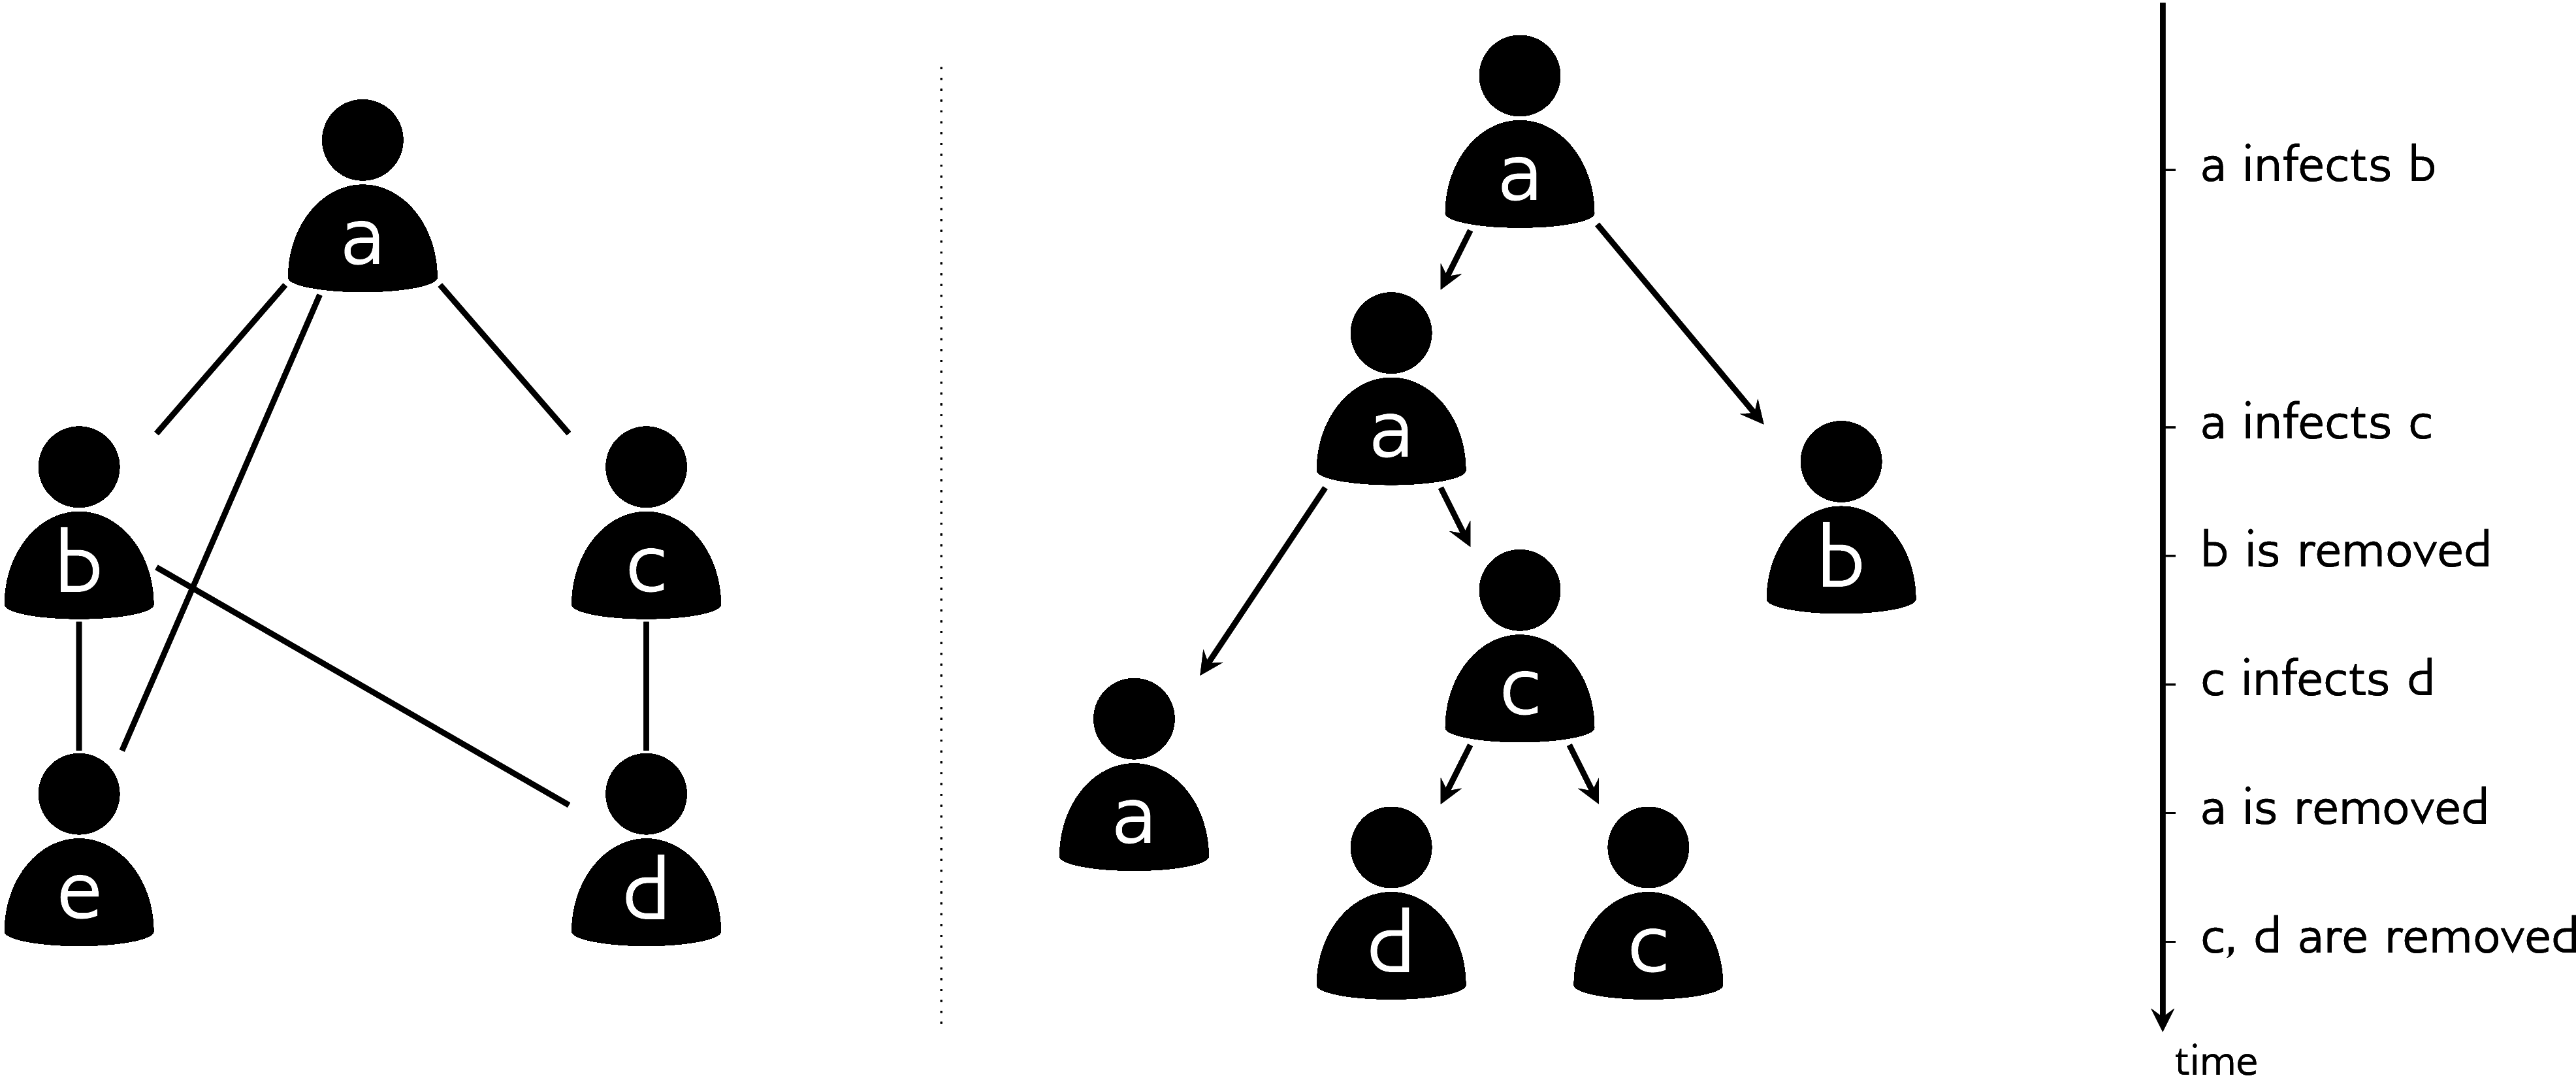
\includegraphics{contactnet}
  \caption[Illustration of a epidemic spread over a contact network]
  {Illustration of epidemic spread over a contact network. On the left, a
   contact network with five hosts, labelled A through E. Directed edges
   indicate six symmetric contacts among the hosts. Coloured, bolded edges
   represent transmissions. The epidemic began with node A, who transmitted to
   nodes B and C. Node C further transmitted to node D, and node E was not
   infected. On the right, the transmission tree topology corresponding to this
   scenario. Note that individual B was sampled before the other infected
   individuals, resulting in a tree with heterochronous tips.}
\end{figure}

\subsection{Models for contact networks}
\label{subsubsec:generative}

Throughout this section, the variable $n$ will be used to refer to the number
of nodes in the network. 

An \defn{Erd\H{o}s-R\'enyi} (ER) network~\autocite{erdos1960evolution}, also
known as a Bernoulli network, was the first network model described. It has a
single parameter, $p$, which is the probability that any particular edge is
present in the network. To construct an ER network, one simply chooses
$p \times \binom{n}{2}$ distinct pairs of nodes and draws an edge between each
pair. The average degree of a node in an ER network is equal to $p \times n$.

A \defn{Barab\'asi-Albert} (BA) network~\autocite{barabasi1999emergence},
incorproates the phenomenon of \defn{preferential attachment} seen in real life
networks. This means that new connections are more likely to involve nodes
which already have a high number of connections - popular nodes tend to become
more popular. In the formulation we consider here, BA networks have two
parameters, $m$ and $\alpha$, which are used to construct the network via the
following algorithm. The network begins as a single node, then the remaining
$n-1$ nodes are added one at a time. Each time a new node is added, it is
connected to $m$ other nodes. The probability of one of these connections
involving an existing node of degree $k$ is proportional to $k^\alpha$. Note
that in the original formulation~\autocite{barabasi1999emergence}, there was an
additional parameter $m_0$ which indicated the number of initial vertices in
the network, and the only value of $\alpha$ considered was 1. For our purposes,
we fix $m_0 = 1$ but allow $\alpha$ to vary. We refer to $\alpha$ throughout
this work as the \defn{preferential attachment power} or just attachment power.

Networks produced by the BA model are \defn{scale free}, which means that the
probability of a node having $k$ connections is proportional to $k^\gamma$ for
some constant $\gamma$. This is also called a \defn{power law} degree
distribution. An important remark on notation must be made here: in network
literature, the Greek letter $\alpha$ has often been used to refer to the power
law exponent of the degree distribution, not the preferential attachment power.
However, the paper defining the network model~\autocite{barabasi1999emergence}
uses $\gamma$ for the power law exponent, and $\alpha$ for the attachment
power, and we shall do likewise. This must be noted because there are reports
in the literature of the power law exponent being as large as 4, which would
seem to conflict with our choice (see subsection XX) to bound $\alpha$ above by
2. The reader should rest assured that it is the attachment power we are
bounding, not the power law exponent.

WS and BA networks differ from ER networks in an important way: it is possible
to explicitly calculate the likelihood of the ER model parameter $p$ given an
observed network, but this cannot be done for the other two models. This is
because the probability of a particular edge occuring is always equal to $p$ in
an ER network, regardless of the presence or absence of any other edges. In
other words, the edges can be viewed as a series of $\binom{n}{2}$ Bernoulli
trials with success probability $p$, so that the likelihood of $p$ given an
observed graph with $k$ edges is distributed as 
Binomial$\left(\binom{n}{2}, p\right)$.

%\section{Approximate Bayesian computation}

%Consider a model $M$, with parameters $\theta$, which we wish to fit to some
%observed data $D$. By ``fit'', we often mean that we want to find particular
%values $\hat{\theta}$ for the parameters which optimize the likelihood of our
%data given those parameters and the model,
%\[
%  \hat{\theta} = \argmax_\theta \Pr(D | M, \theta).
%\]
%This $\hat{\theta}$ is the \defn{maximum likelihood} parameter estimate. Note
%that we are employing a common abuse of notation here, where $\Pr(\cdots)$ is
%being unsed to refer to a probabilty \emph{density} rather than a true
%probability. Alternative to maximum likelihood, we may be interested less in a
%point estimate and more in the posterior distribution of possible values of
%$\theta$ given our data, $\Pr(\theta \mid M, D)$. This will be expanded upon
%below, but for the moment, for illustrative purposes, we restrict our attention
%to the maximum likelihood problem.
%
%If the model we are fitting is sufficiently simple, it may be possible to
%calculate $\hat{\theta}$ directly, using calculus. Most models do not admit
%analytic maximum likeilhood solutions, but if the likelihood any set of
%parameters can be calculated up to a normalizing constant, then
%${\Pr(D \mid M,\theta)}$ can be optimized numerically. A wide range of
%optimization strategies exist, the choice of which to use depending on the
%complexity of the model and whether or not we have access to the gradients of
%the likelihood function with respect to each of the parameters. The majority of
%modelling problems fit into this category, and numerical optimization is
%well-developed and extremely widely used.
%
%However, there are some cases, often when the observed data is of a complex
%type, that explicitly calculating the likelihood of some observed data is
%impossible, even up to a normalizing constant. For example, suppose that we
%want to model a chess player's behaviour. We will set up a simple one-parameter
%model which describes the chess playing process.  The parameter, $a \in [0, 1]$
%indicates the player's eagerness to remove his opponent's pieces from the
%board. We can write down an algorithm for the player's behaviour under such a
%model.
%
%% TODO: don't break this over the page
%
%\begin{algorithmic}
%  \While{the game is not over}
%    \If{I can capture an opponent's piece and $\Uniform(0, 1) < a$}
%      \State{capture the piece}
%    \Else
%      \State{make any other move at random}
%    \EndIf
%  \EndWhile
%\end{algorithmic}
%
%Suppose the observed data are the ending configurations of the board, after the
%player has concluded a game against an opponent with a known value of $a$. The
%model we have designed is very simple, but it is not obvious how to calculate
%the likelihood of a particular ending configuration. Indeed, it seems that the
%only way is to enumerate every possible path the game could have taken, and
%tabulate the ending configurations of each. Clearly, this is infeasible.
%Approximate Bayesian computation was designed for situations like these, where
%exact likelihoods are not available, perhaps due to the model involving an
%algorithm or generative process.

\section{Approximate Bayesian computation}

\subsection{Overview and motivation}

\gls{ABC} is the name for a family of techniques which can be used to fit
complex models to observed data. We shall make this precise below, but to fully
describe and motivate \gls{ABC}, it is necessary to first make explicit exactly
what we mean by ``fitting'' a model. 

A linear regression is a model of the relationship between some data points
$\vec{x} = (x_1, \ldots, x_n)$ and outcomes $\vec{y} = (y_1, \ldots, y_n)$.
This model assumes that the outcomes are linearly related to the data, modulo
some noise caused by measurement errors, environmental fluctuations, and so on.
In other words, there is a constant $b$ such that $y_i = bx_i + \varepsilon_i$,
where $\varepsilon_i$ is the error associated with the outcome $y_i$. If we
make the additional assumption that the errors are normally distributed, then
the model takes the form
\begin{align}
  y_i = bx_i + \N(0, \sigma^2).
  \label{eq:regression}
\end{align}
When we say that we want to fit this model to observed data, we mean that we
want to find particular values for $b$ and $\sigma$ which are in some way
optimal given $\vec{x}$ and $\vec{y}$. We shall make this precise below. Notice
that, if we fix $b$ and $\sigma$, then we can write down the probability density
of observing $y_i$ given $x_i$. If $f_\N(\cdot \mid \mu, \sigma)$ is the
\gls{pdf} of the normal distribution with mean $\mu$ and variance $\sigma^2$,
and the $y_i$ are all independent, then
\[
  f(\vec{y} \mid \vec{x}, b, \sigma) = 
  \prod_{i=1}^n f_\N(y_i - bx_i \mid 0, \sigma^2).
\]
This gives us a natural criterion for choosing the optimal parameters: we want
to pick $b$ and $\sigma$ which define a model where the probability density of
our observed data is as high as possible. When performing such an optimization,
the above density function is also called the \defn{likelihood} of the
parameters,
\[
  \L(b, \sigma \mid \vec{x}, \vec{y}) = f(\vec{y} \mid \vec{x}, b, \sigma).
\]
The particular $b$ and $\sigma$ which optimize $\L(b, \sigma)$ are called the
\gls{ML} estimates.

%Mathematical models can be grouped into three categories in terms of our
%ability to fit them to observed data. First, there is a limited set of models
%which can be fit explicitly by using calculus to minimize a loss function. The
%canonical example of this type of model is a linear regression. 
%Notice that, if we fix $b$, then since $y_i$ and $x_i$ are both given,
%$\varepsilon_i$ is also fixed. The process of fitting a linear model means
%choosing the ``best'' $b$. For least squares, this optimal $b$ is defined as
%the one which minimizes the sum of the squared $\varepsilon_i$. 

Now that we have defined what it means to fit a least-squares linear
regression, there remains the question of how to go about finding this optimal
$b$ value. Recall that the errors $\varepsilon_i$ are fixed for a particular
$b$, and our objective is to minimize the loss function, which is the sum of
the squared errors. Naively, we could simply try many different $b$ values,
calculate the loss function for each, and choose the $b$ which gives the
smallest value. This approach, though basic, falls under the umbrella of
\defn{numerical optimization}, which is the most common way the majority of
models are fit. Of course, there is a whole field devoted to more sophisticated
methods for exploring the parameter space, but they all boil down to the basic
method of trying different values and choosing the one which minimizes the
loss.

In the case of least-squares linear regression, there is another method we
could use. Looking at equation~\ref{eq:regression} for the model, it is easy to
rearrange terms to solve for $\varepsilon_i$ in terms of the other variables:
we get $\varepsilon_i = y_i - bx_i$. In fact, we can write down the entire loss
function, which is the sum of the squared $\varepsilon_i$ in terms of $b$:
\[
  \sum \varepsilon_i^2 = \sum (y_i - bx_i)^2,
\]
where the sums are over all $i$ from 1 to $n$, the number of points in the data
set. We will not describe the procedure here, but it is possible to explicitly
minimize the right-hand side by finding the point where the derivative with
respect to $b$ is zero. However, the method of directly minimizing the loss
function with calculus is only applicable to a very narrow class of simple
models. For the majority, the loss function is too complicated to set the
derivative with respect to the parameters to zero and solve.

Because of the limited space of models which permit exact solutions, numerical
optimization of a loss function is the most frequently used method to fit a
model. 

An approximate Bayesian computation approach to least-squares regression might
be as follows. We will need to make an additional assumption: that the errors
$\varepsilon_i$ are normally distributed. That is, our linear model is now of
the form
\[
  y_i = bx_i + \N(0, \sigma),
\]
where $\N(0, \sigma)$ indicates a normal distribution with mean zero and
variance $\sigma$. We do not know $\sigma$ in advance, so this is another
parameter we will need to estimate. There is nothing special about normal
distributions - we could have chosen any other distribution we deemed
appropriate. 

The main idea of approximate Bayesian computation is that the ``best''
parameters will define a model which produces simulated data similar to the
real data. Suppose we fix values of $b$ and $\sigma$. Then, using the given
data points $x_i$, we can generate simulated observations $y_i^*$ by adding
$bx_i$ and a randomly chosen error drawn from $\N(0, \sigma)$.

\subsection{Algorithms for ABC}
\label{subsubsec:abcalg}

Approximate Bayesian computation does not refer to a particular procedure for
model fitting. Rather, ABC refers to the general strategy of choosing model
parameters based on the resulting model's propensity to generate data
resembling the real data. There are three main classes of ABC algorithm which
have been developed so far: rejection, \gls{MCMC}, and sequential Monte Carlo
(SMC). 

All of these approaches require some common elements. First, as with all
Bayesian methods, we are required to specify a \defn{prior distribution},
denoted $\pi$, on the parameter space. The prior specifies what we already know
or believe about the model parameters. Second, in order to compare simulated to
observed data, we need to be able to summarize a data set in a numerical
format. This is accomplished by a function, denoted $\eta$, which computes a
vector of hopefully informative summary statistics on a data set. Third, we
need a distance function $\rho$ which tells us how similar two data sets are to
each other, based on their summary statistics.

Continuing with the linear model example, we need to specify a prior $\pi(a, b,
\sigma)$ on the three parameters. We do not have much certain information about
these parameters except that $\sigma$ has to be at least zero, but it seems
reasonable to assume that extreme relationships are fairly rare, and that
positive and negative correlations are equiprobable. Therefore, we will let
$a$, $b$, and $\sigma$ be independent, $a$ and $b$ be normally distributed,
and $\sigma$ be log-normally distributed. That is,
\[
  \pi(a, b, \sigma) = 
  \begin{cases}
    \Pr[\N(0, 1) = a] \cdot \Pr[\N(0, 1) = b] \cdot \Pr[\N(0, 1) = \log\sigma]
     & \sigma > 0 \\
    0 & \sigma \le 0.
  \end{cases}
\]
For the vector of summary statistics, we will use the mean and variance of the
simulated data,
\[
  \eta(\vec{y}) = \left<\E[\vec{y}], \Var[\vec{y}]\right>.
\]
Finally, for the distance function $\rho$ we take the standard Euclidian
distance.

Rejection ABC is the simplest method, and also the one which was first
proposed~\autocite{rubin1984bayesianly}. Effectively, it comes down to the
approach described in the previous subsection of guessing parameter values
until one is close enough to the truth. More specificially, a possible set of
parameters $\theta$ is drawn from the prior distribution, and a simulated data
set $z$ is generated from the model with those parameters. If the distance
between the simulated data set and the real data, $\rho(\eta(y), \eta(z))$, is
small enough, then we accept $\theta$ as a sample from the posterior. This can
be repeated until as many samples as desired are obtained.

% MCMC
The second method is \gls{ABC}-\gls{MCMC}. This is similar to ordinary Bayesian
\gls{MCMC}, except that a ratio of distances to the observed data replaces the
likelihood ratio. The algorithm begins by sampling a single vector of parameter
values $\theta$ from the prior distribution $\pi(\theta)$. It then proceeds
iteratively: a new parameter vector $\theta^*$ is chosen according to a
proposal distribution $q(\theta^* \mid \theta)$. The proposal distribution $q$
is often taken to be a Gaussian centred at $\theta$. Then $\theta^*$ is
accepted as the new $\theta$ with probability
\[
  \max\left(1, \text{TODO} \right),
\]
or discarded otherwise. This process is iterated until some stopping criterion
is reached, typically a simple limit on the number of steps. After some initial
number of iterations, known as \defn{burn-in}, parameters $\theta$ are
routinely sampled. Since points in parameter space are visited in proportion to
their posterior probability, these samples can be taken to approximate the
posterior distribution on $\theta$, and can be used to calculate point
estimates and confidence intervals.

The most recently developed class of algorithms for ABC is sequential
Monte-Carlo (SMC)~\autocite{sisson2007sequential}. As with the other two
classes, we want to eventually obtain a sample from the posterior distribution
$f(\theta \mid D)$. The idea of SMC is to begin with a sample from a
distribution we know, most often the prior, and approach the posterior smoothly
by progressing through a series of intermediate distributions.

